%!TeX root=../tese.tex
%(dica para o editor de texto: este arquivo é parte de um documento maior)
% para saber mais: https://tex.stackexchange.com/q/78101/183146

% https://otexts.com/fpp2/index.html
% https://www.tensorflow.org/tutorials/structured_data/time_series

\chapter{Séries temporais}
\label{cap:series}

O segundo objetivo deste trabalho é testar a utilização das redes neurais na previsão de séries temporais financeiras, e para isso são apresentados neste capítulo os conceitos básicos de séries temporais. Também são discutidos brevemente os modelos tradicionais de análise e descrição das séries, ou de previsões de valores futuros, de acordo com o objetivo do estudo. Tais modelos são, por exemplo, baseados em médias móveis, tendências e sazonalidades presentes nos dados.

De acordo com Pedro A. Morettin e Clélia M C. Toloi \citep{morettin}, uma série temporal é qualquer conjunto de observações ordenadas no tempo. São exemplos: valores diários de poluição de uma cidade, valores mensais de temperatura, índices diários da bolsa de valores, número médio anual de manchas solares e registro de marés em portos e estuários.

A análise e predição de cotações de moedas estrangeiras, índices de ações, entre outros dados econômicos, constituem uma área essencial da economia e que exige a avaliação de um número enorme de fatores, muitos dos quais de características humanas e portanto imprevisíveis em sua exatidão, sendo descritos como exemplos de fenômenos \emph{estocásticos}, isto é, probabilísticos.

As séries temporais podem ser \defi{contínuas} em função do tempo, como é o exemplo de registros de marés, ou \defi{discretas} como são todos os outros exemplos, ou seja, os valores são tomados a $N$ intervalos regulares de um período $T$ considerado, tal que $N = T/\Delta t$. Na prática, para o uso em modelos, segundo explica Morettin e Toloi \citep{morettin}, as séries contínuas devem ser discretizadas em intervalos, uma vez que é esse tipo de dado que poderá ser processado num computador.

Pode-se classificar a análise das séries temporais de acordo com seu objetivo de estudo. Morettin e Toloi \citep{morettin} listam os alguns objetivos principais:

\begin{itemize}
	\item{Investigar o mecanismo gerador da série temporal, procurando descrevê-la a partir de uma função teórica.}
	\item{Fazer previsões de valores futuros da série, seja tanto a curto quanto a longo prazo.}
	\item{Descrição da série, em termos de tendências, variações sazonais, ou então análises descritivas por meio de histogramas, médias móveis, etc.}
	\item{Procurar por periodicidades relevantes nos dados, quando não fazemos suposições de periodicidades comuns como semanais, mensais ou anuais, por exemplo.}
\end{itemize}

Neste contexto, Morettin e Toloi \citep{morettin} definem que um modelo é uma descrição probabilística de uma série temporal, cabendo ao cientista de dados decidir a melhor utilização desse modelo segundo seus objetivos. 

Além disso eles afirmam que qualquer tarefa de previsão, sendo este o objetivo, será baseada em algum procedimento computacional que calcula uma estimativa do futuro baseada na otimização de uma função de perda calculada sobre combinações lineares de valores do passado. É a união de um modelo probabilístico com a otimização de uma função de perda que define um \defi{método de previsão}.

Há dois tipos básicos de modelos que lidam com séries temporais, de acordo com Morettin e Toloi \citep{morettin}, que são os modelos \defi{paramétricos}, onde a análise é feita no \emph{domínio temporal} com suposições e parâmetros a serem estimados, e os modelos \defi{não-paramétricos}, em que a análise é feita no \emph{domínio das frequências} com um enfoque mais descritivo e sem muitas suposições.

Dentre os modelos paramétricos, destacam-se os modelos \emph{ARIMA} (\emph{autorregressivos integrados de médias móveis}), disponíveis como bibliotecas das linguagens \eng{Python} e \eng{R}, enquanto que entre os modelos não-paramétricos destaca-se a \emph{análise espectral}, também denominada de \emph{análise de Fourier}, já que as ferramentas utilizadas são as transformadas de Fourier e suas variações.

\section{Processos estocásticos}

De acordo com Morettin e Toloi \citep{morettin}, um \defi{processo estocástico} é uma família $Z = \{ Z(t), t \in \mathcal{T} \}$, onde o conjunto $\mathcal{T}$ é normalmente tomado como $\mathcal{T} = \mathbb{Z}$ ou $\mathcal{T} = \mathbb{R}$, tal que, para cada $t \in \mathcal{T}$, $Z(t)$ é uma variável aleatória (v.a.). 

Portanto, um processo estocástico é uma família de variáveis aleatórias reais $Z(t),\; t \in \mathcal{T}$, definidas num mesmo espaço de probabilidades $(\Omega, \mathcal{A}, \mathcal{P})$, e portanto $Z(t)$ é uma função de dois argumentos, isto é, $Z(t, \omega),\; t \in \mathcal{T},\; \omega \in \Omega$.

Para cada $t \in \mathcal{T}$ fixado, $Z(t, \omega)$ será uma v.a. com uma distribuição de probabilidades. Pode haver uma função de densidade de probabilidade diferente para cada $t \in \mathcal{T}$, mas normalmente assume-se que é a mesma, conforme anotado por Morettin e Toloi \citep{morettin}.

Por outro lado, para cada $\omega_i \in \Omega$ fixado, denotamos $Z(t, \omega_i)$ por $Z^{(i)}(t)$ como uma função de $t$, denominada de \defi{trajetória} do processo, ou simplesmente de \emph{série temporal}. Isto define uma série temporal como uma trajetória ou realização de um processo estocástico, o que pode ser melhor ilustrado pela Figura \ref{fig:trajetorias}, abaixo.

\begin{figure}[htb]
\centering
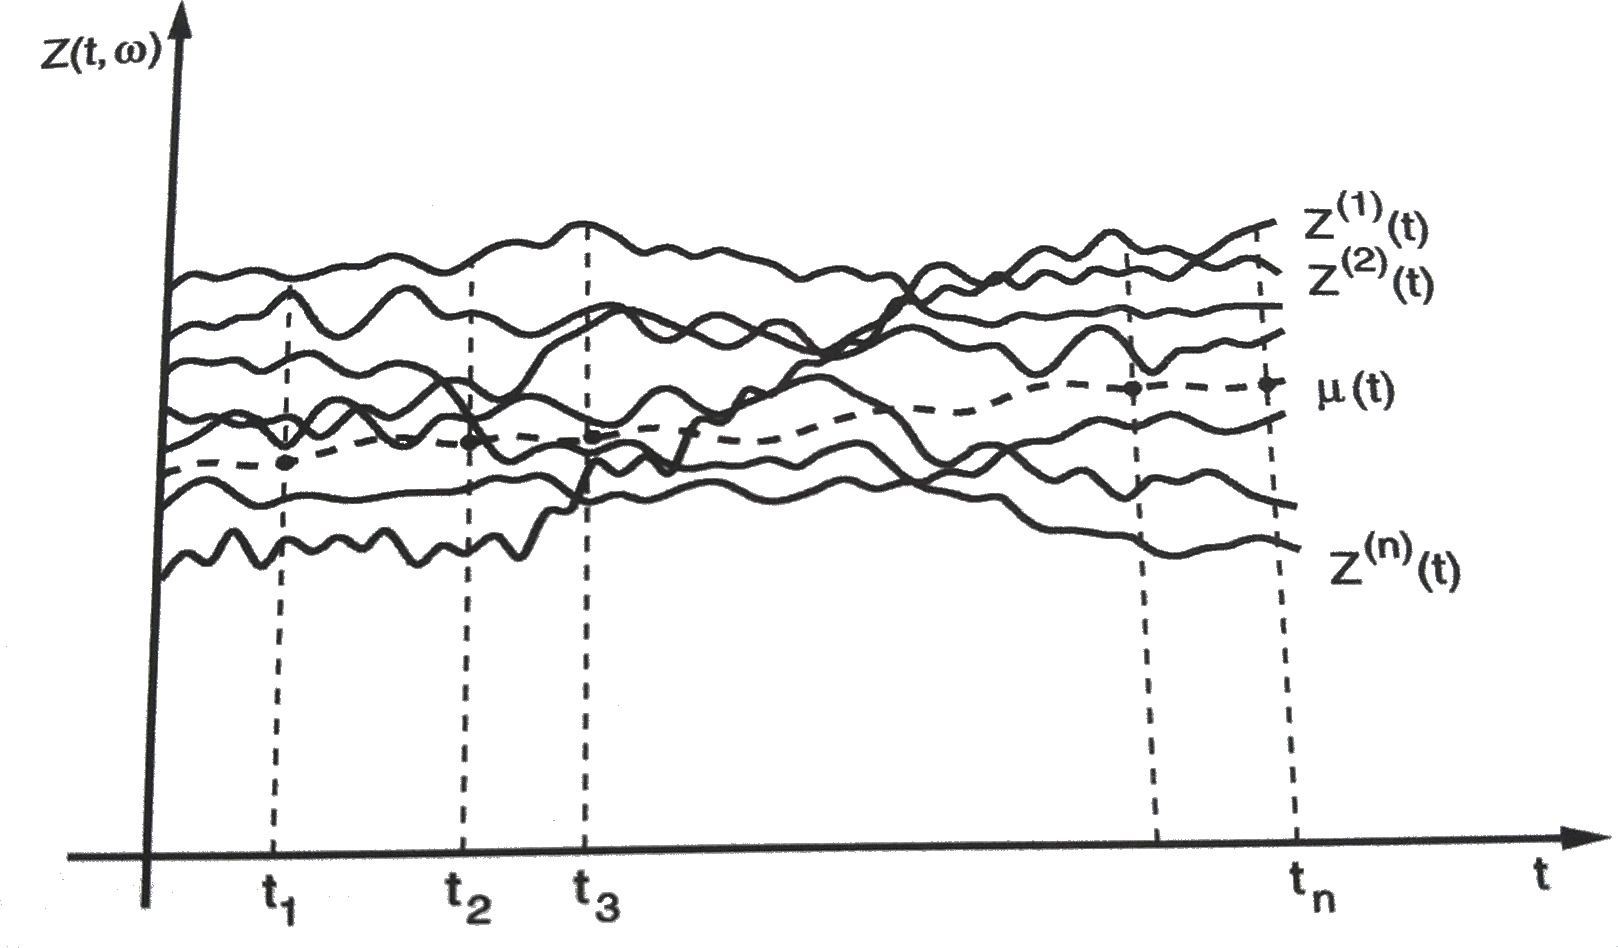
\includegraphics[width=10cm]{figuras/trajetorias}
\caption{Processo estocástico como uma família de trajetórias, isto é, de séries temporais.\footnote{  de \citep{morettin}, pág 27.}}
\label{fig:trajetorias}
\end{figure}

Estaremos interessados em processos univariados tanto em $\mathcal{T}$ quanto em $\Omega$, isto é, séries temporais de apenas um argumento temporal, e com um evento $\omega \in \Omega$ fixado e portanto omitido, o que simplifica a notação de $\{Z^{(i)}(t), t \in \mathcal{T}\}$ para $\{Z(t), t \in \mathcal{T}\}$, o que definem as \emph{séries temporais univariadas}, que descrevem como uma v.a. real evolui no domínio temporal $\mathcal{T}$.

Além disso, para as séries e modelos aqui tratados iremos restringir $\mathcal{T} = \mathbb{Z}$, assim omitiremos a definição de um domínio geral e fixaremos a notação como sendo $\{Z(t), t \in \mathbb{Z}\}$ ou ainda $\{Z_t, t \in \mathbb{Z}\}$, para denotar as \emph{séries temporais discretas univariadas}, que além de discretas são equidistantes no tempo. A partir de agora, serão chamadas simplesmente de \defi{séries temporais}, pois são os únicos processos estocásticos de interesse neste trabalho.

\subsection{Definições}

Seguem algumas definições que nos levarão a classes específicas de processos estocásticos, com as quais lidaremos daqui em frente. Sejam $t_1, \ldots, t_n$ elementos quaisquer de $\mathcal{T}$, daí se conhecermos as \defi{distribuições finito-dimensionais} de $Z$ dadas por:

\begin{equation}\label{series:2.1}
F(z_1, \ldots, z_n; t_1, \ldots, t_n) = P\{ Z_{t_1} \leq z_1, \ldots, Z_{t_n} \leq z_n \}
\end{equation}

Teremos então que o processo estocástico $Z = \{ Z_t, t \in \mathcal{T} \}$ estará especificado, para todo $n \geq 1$. Tais funções de distribuição devem, de acordo com Morettin e Toloi \citep{morettin} satisfazer as condições:

	(i) (Simetria) Para qualquer permutação $j_1, \ldots, j_n$ dos índices $1, \dots, n$:
\[ F(z_{j_1}, \ldots, z_{j_n}; t_{j_1}, \ldots, t_{j_n}) = F(z_1, \ldots, z_n; t_1, \ldots, t_n) \]

	(ii) (Compatibilidade) Para $m < n$:
\[ \lim_{\mathlarger{z_{m+1} \to \infty, \ldots, z_n \to \infty}} F(z_1, \ldots, z_m, z_{m+1}, \ldots, z_n; t_1, \ldots, t_n) = F(z_1, \ldots, z_m; t_1, \ldots, t_m) \]

Segundo Morettin e Toloi \citep{morettin}, pode-se demonstrar que qualquer conjunto de funções de distribuição da forma (\ref{series:2.1}) satisfazendo as duas condições acima define um processo estocástico $Z$ sobre $\mathcal{T}$.

Em termos práticos, não se conhecem as funções de distribuição finito-dimensionais de um processo $Z$ sobre $\mathcal{T}$. Assim a abordagem mais utilizada, conforme Morettin e Toloi \citep{morettin} é tentar determinar os momentos, principalmente os de primeira e segunda ordem, das v.a. $Z_{t_1}, \ldots, Z_{t_n}$. 

O momento de primeira ordem, isto é, a \defi{média} de $Z$ é definida por: 

\begin{equation}\label{series:2.5}
\mu(1; t) = \mu(t) = \E\{Z(t)\} = \int_{-\infty}^{\infty} z f(z;t)dz, t \in \mathcal{T}
\end{equation}

Define-se, a partir dos momentos de primeira ordem, a \defi{função de autocovariância} (\emph{facv}) de $Z$:

\begin{equation}\label{series:2.6}
\gamma(t_1, t_2) = \mu(1,1; t_1,t_2) - \mu(1; t_1)\mu(1; t_2) = \Cov\{Z(t_1),Z(t_2)\}
\end{equation}

Particularmente, quando $t = t_1 = t_2$, define-se a função \defi{variância} de $Z$, configurando um momento de segunda ordem, por:

\begin{equation}\label{series:2.7}
\gamma(t, t) = \Var\{Z(t)\} = \E\{Z^2(t)\} - \E^2\{Z(t)\}
\end{equation}

\subsection{Processos estacionários}

Um processo $Z$ é dito \defi{estacionário} se suas características para qualquer tempo não dependem da escolha da origem do domínio temporal, isto é, as características de $Z(t + \tau)$ para todo $\tau$, são as mesmas de $Z(t)$. Morettin e Toloi \citep{morettin} nomeia o parâmetro $\tau$ de ``\defi{lag}''\footnote{jargão em inglês que em português pode significar latência ou atraso.}, e dá como exemplo de processo estacionário as medidas de vibrações de um avião em regime estável de vôo.

Formalmente, um processo estocástico $Z = \{Z(t), t \in \mathcal{T}\}$ é \defi{fracamente estacionário} ou estacionário de segunda ordem, se e somente se:

	(i) $\E\{Z(t)\} = \mu(t) = \mu, \;\;\; \forall ~ t \in \mathcal{T};$

	(ii) $\E\{Z^2(t)\} < \infty, \;\;\; \forall ~ t \in \mathcal{T};$

	(iii) $\gamma(t_1, t_2) = \Cov\{Z(t_1), Z(t_2)\}$ é uma função de $|t_1 - t_2|, \;\;\; \forall~ t_1, t_2 \in \mathcal{T}.$

Dessa forma, podemos dizer que processos estacionários de segunda ordem desenvolvem-se em torno de uma média constante, ou seja, ao redor de uma mesma tendência ou reta. É possível citar dois tipos de não-estacionariedade. 

Existem os processos \emph{homogêneos}, que apresentam uma estacionariedade inicial mas que depois sofrem uma mudança de tendência e então tornam-se estacionárias novamente, mas não necessariamente ao redor da mesma média inicial, e que segundo Morettin e Toloi \citep{morettin} podem se tornar estacionários se tomarmos diferenças sucessivas da série original.

Tomar diferenças de uma série $Z(t)$ corresponde a criar uma nova série a partir da original. A primeira diferença de $Z(t)$ é definida por:

\begin{equation}\label{series:2.12}
\Delta Z(t) = Z(t) - Z(t - 1)
\end{equation}

Recursivamente, a partir dessa primeira definição, podemos escrever a n-ésima diferença de $Z(t)$ como sendo:

\begin{equation}\label{series:2.13}
\Delta^n Z(t) = \Delta[\Delta^{n-1} Z(t)]
\end{equation}

Adicionalmente, aplicar a transformação não-linear $\log Z(t)$ também pode ser útil para transformar uma série não-estacionária em uma série estacionária. De acordo com Morettin e Toloi \citep{morettin}, a transformação logarítmica é muito usada em séries econômicas e será apropriada se a variância da série for proporcional à média.

Para exemplificar esses conceitos, considere a Figura \ref{fig:exe_estac}. Temos à esquerda uma série temporal que é uma realização de um processo não-estacionário homogêneo, a saber, índices mensais da bolsa de valores Ibovespa. À direita, foi aplicado o logaritmo da primeira diferença da série, o que gerou uma série estacionária.

\begin{figure}[htb]
\centering
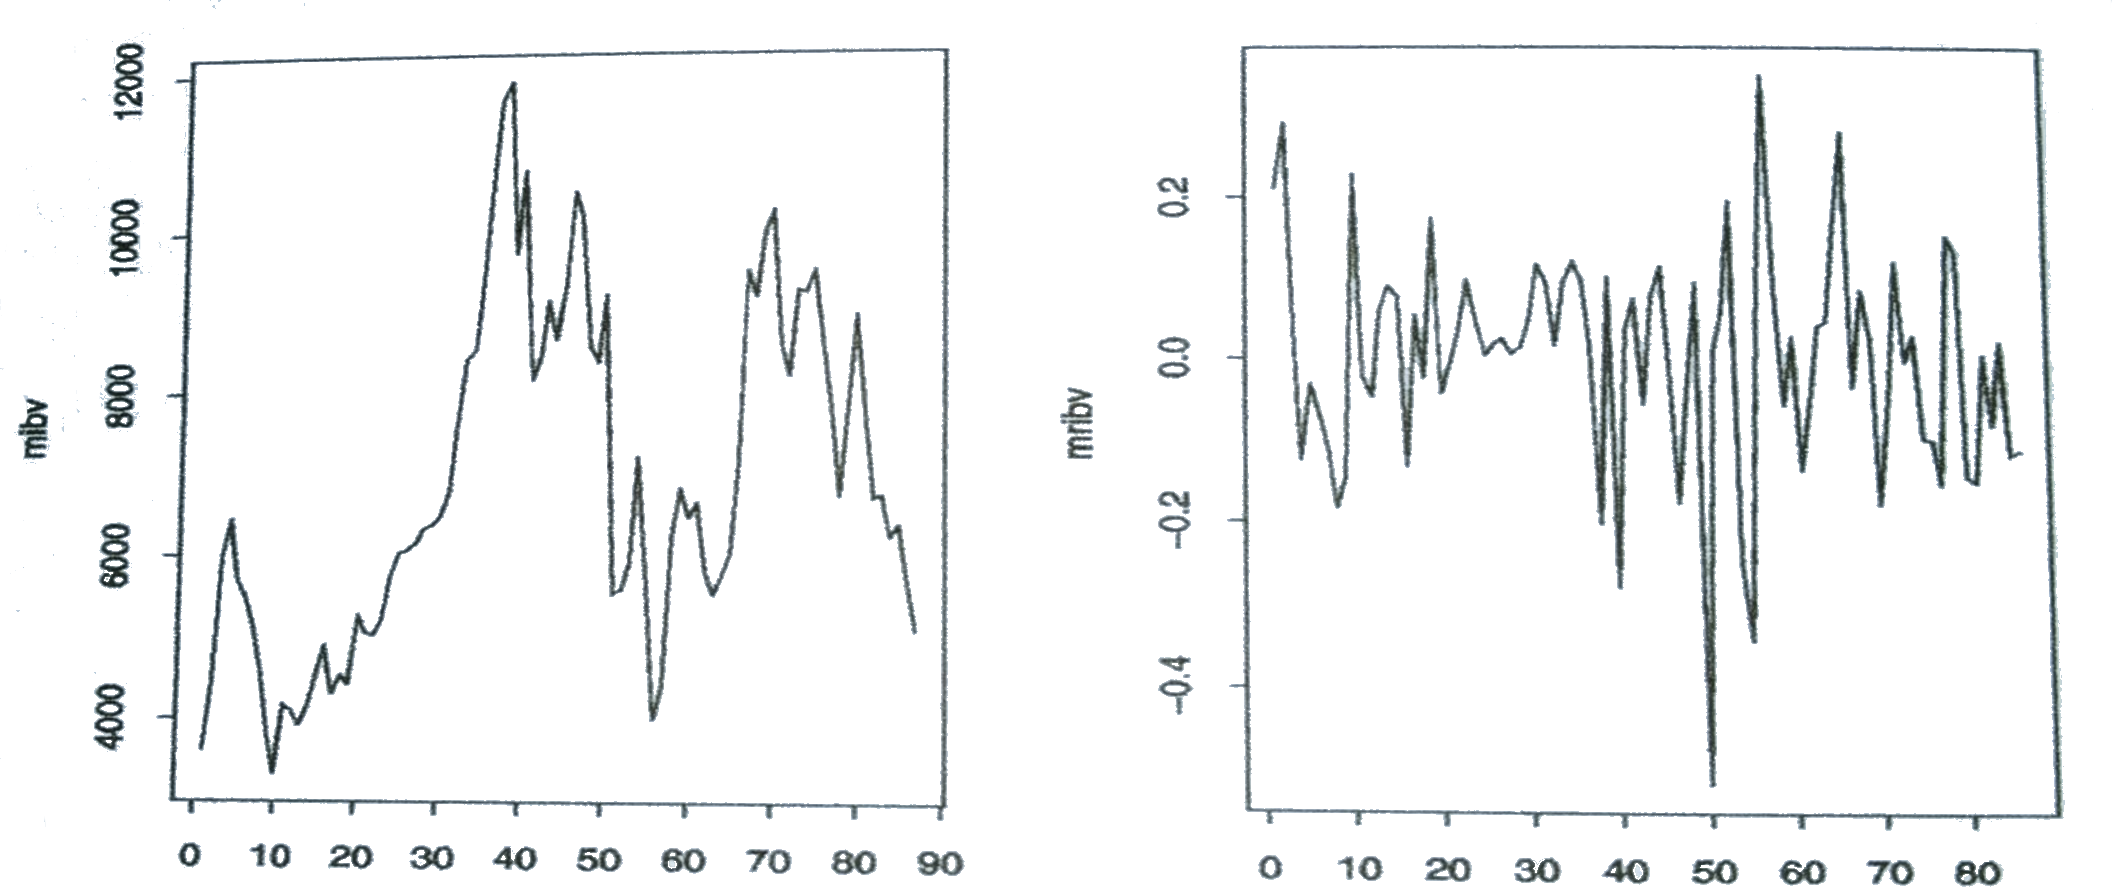
\includegraphics[width=14cm]{figuras/exemplo_estac}
\caption{Esquerda: Índices mensais do Ibovespa. Direita: Log-diferença do Ibovespa.\footnote{Extraído de \citep{morettin}, pág 7.}}
\label{fig:exe_estac}
\end{figure}

O segundo tipo de não-estacionariedade é chamada de \emph{explosiva}. Um exemplo de um processo não-estacionário explosivo é uma série temporal que descreve o crescimento de uma população de bactérias. Não tratamos de processos deste tipo neste trabalho.

\subsection{Função de autocorrelação}

Seja $\{ X_t, t \in \mathbb{Z} \}$ um processo estacionário real com tempo discreto, de média $\mu = 0$ e \emph{facv} $\gamma_\tau = \E\{ X_t, X_{t+\tau} \}$. Sob essas condições, Morettin e Toloi \citep{morettin} demonstram que a \emph{facv} $\gamma_\tau$ satisfaz as propriedades:

	(i) $\gamma_0 > 0$,

	(ii) $\gamma_{-\tau} = \gamma_\tau$,

	(iii) $|\gamma_\tau| \leq \gamma_0$,

	(iv) $\sum_{j=1}^n \sum_{k=1}^n a_j a_k \gamma_{\tau_j - \tau_k} \geq 0 \;\;\; \forall a_1, \ldots, a_n \in \mathbb{R}$ e $\tau_1, \ldots, \tau_n \in \mathbb{Z}$,

	(v) $\lim_{|\tau| \to \infty}  \gamma_\tau = 0$.

Define-se a \defi{função de autocorrelação} (\emph{fac}) de um processo estocástico por:

\begin{equation}\label{series:2.14}
\rho_\tau = \frac{\gamma_\tau}{\gamma_0}
\end{equation}

A \emph{fac} de um processo estacionário possui todas as propriedades da \emph{facv} acima listadas e, em particular, $\rho_0 = 1$. O mais interessante é a ressalva de Morettin e Toloi \citep{morettin} de que a recíproca é verdadeira, isto é, dado um processo cuja \emph{fac} ou \emph{facv} possuem essas propriedades, então ele é estacionário. Dessa forma, temos um arcabouço teórico que nos permite investigar a existência da propriedade estacionária de uma série temporal dada.

\subsection{Exemplos de processos estocásticos}

O exemplo mais simples é o de uma \emph{sequência aleatória}. Uma sequência de v.a. definidas num mesmo espaço amostral $\Omega$ dada por $\{ X_n , n = 1, 2, \ldots \}$ é um processo estocástico com parâmetro discreto, ou seja, $\mathcal{T} = \{ 1, 2, \ldots \}$. Para todo $n \geq 1$ temos, em geral, que:

\[ P\{X_1 = a_1, \ldots, X_n = a_n\} = P\{X_1 = a_1\}\times P\{X_2 = a_2|X_1 = a_1\} \]
\[ \times\ldots\times P\{X_n = a_n|X_1 = a_1, \ldots, X_{n-1} = a_{n-1}\}\]

Se simplificarmos esse caso geral para o caso de uma sequência $\{ X_n , n \geq 1 \}$ de v.a. \emph{mutuamente independentes} então:

\[ P\{X_1 = a_1, \ldots, X_n = a_n\} = P\{X_1 = a_1\}\times\ldots\times P\{X_n = a_n\} \]

E se, além disso, todas as v.a. dessa sequência tiverem a mesma distribuição de probabilidades, elas serão portanto independentes e identicamente distribuídas (i.i.d.), o que configura $X_n = \{ X_n , n \geq 1 \}$, uma sequência de v.a. i.i.d., como um processo estocástico estacionário.

Definindo $\E\{X_n\} = \mu$, $\Var\{X_n\} = \sigma^2$, para todo $n \geq 1$, teremos que a \emph{facv} de $X_n$ será dada por:

\begin{equation}\label{series:2.19}
\gamma_\tau = \Cov\{X_n, X_{n+\tau}\} = \left\{\begin{array}{lr} \sigma^2, & \text{ se } \tau = 0 \\ 0, & \text{ se } \tau \neq 0 \end{array}\right.
\end{equation}

E, a \emph{fac} de $X_n$, será tal que:

\begin{equation}\label{series:2.20}
\rho_\tau = \left\{\begin{array}{lr} 1, & \text{ se } \tau = 0 \\ 0, & \text{ se } \tau \neq 0 \end{array}\right.
\end{equation}

Um segundo exemplo de processo estocástico, e muito mais útil para os estudos de séries temporais, é o de \defi{ruído branco}. Morettin e Toloi \citep{morettin} definem que a sequência $\{\epsilon_t,\; t \in \mathbb{Z}\}$ é um \emph{ruído branco discreto} se as v.a. $\epsilon_t$ não são correlacionadas, ou seja, $\Cov\{\epsilon_t, \epsilon_s\} = 0, t \neq s$.

Esse processo será estacionário se $\E\{\epsilon_t\} = \mu_\epsilon$ e $\Var\{\epsilon-t\} = \sigma_\epsilon^2$, para todo $t \in \mathbb{Z}$. Dessa forma, as \emph{facv} e \emph{fac} de um ruído branco serão dadas, respectivamente e analogamente, por (\ref{series:2.19}) e (\ref{series:2.20}). Tipicamente representa-se o gráfico de uma função de autocorrelação conforme o exemplo do \emph{fac} de um ruído branco, dado na Figura \ref{fig:fac_ruido}.

\begin{figure}[htb]
\centering
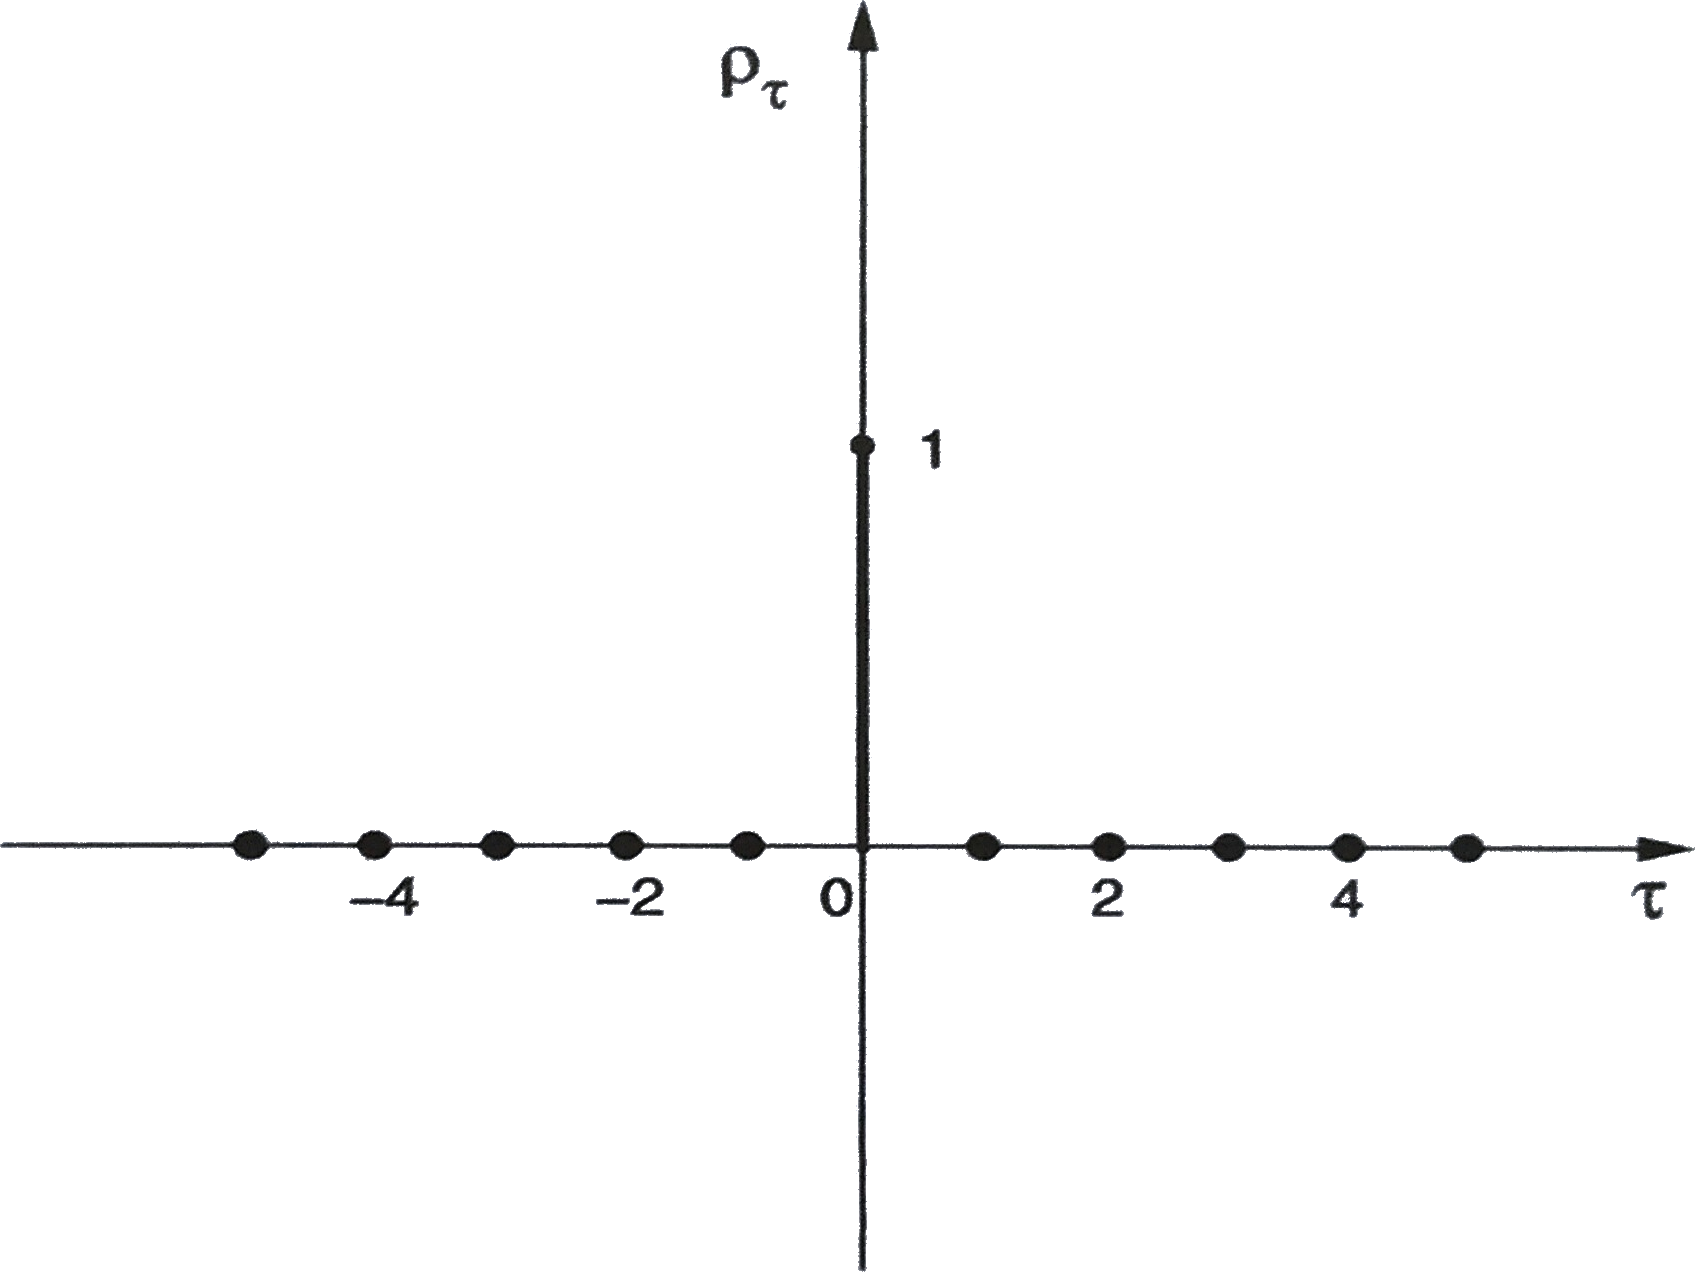
\includegraphics[width=8cm]{figuras/fac_ruido}
\caption{Função de autocorrelação (\emph{fac}) de um ruído branco.\footnote{Extraído de \citep{morettin}, pág 35.}}
\label{fig:fac_ruido}
\end{figure}

Normalmente, é dito por Morettin e Toloi \citep{morettin} que, sem perda de generalidade, podemos assumir que a média de um ruído branco é zero. E, assim, escrevemos:

\[ \epsilon_t \sim RB (0, \sigma_\epsilon^2). \]

Se, as v.a. de $\epsilon_t$ forem independentes, então é um resultado de probabilidade conhecido e citado por Morettin e Toloi \citep{morettin} que serão também não correlacionados. Um ruído branco, como definido acima, e com a propriedade adicional da independência, é um terceiro exemplo de um processo estocástico, chamado de \emph{processo puramente aleatório}. Nesse caso, escrevemos:

\[ \epsilon_t \sim i.i.d. (0, \sigma_\epsilon^2). \]

Outros exemplos de processos estocásticos que podemos citar, menos formais e mais físicos, são os \emph{passeios aleatórios}, que fazem por exemplo, a modelagem de um sistema de partículas livres, como as moléculas de um gás ideal. E, outro exemplo, análogo, é o do \emph{movimento browniano}, que modela, por exemplo, como partículas de poeira movimentam-se num fluído visto como um conjunto de muitas moléculas ligadas entre si, como a água no estado líquido.

\section{Os modelos ARIMA}

Já foi citado acima que existem os modelos parâmétricos, que lidam com as séries no domínio temporal, e os modelos não-paramétricos que lidam com o \defi{espectro} da série, isto é, o conjunto das frequências da série, onde as componentes desse espaço das frequências são ortogonais entre si, o que garante a não correlação entre as frequências, diferindo dos valores sob o domínio temporal que quase sempre são correlacionados entre si, conforme explicado por Morettin e Toloi \citep{morettin}.

Se temos uma série temporal discreta $Z = \{ Z_t, t \in \mathbb{Z} \}$, que assumimos ser um processo estacionário, e assumindo também que as autocovariâncias $\gamma_\tau$ são tais que $\sum_{\tau=-\infty}^{\infty} |\gamma_\tau| < \infty$, então o espectro de $Z$, isto é, a \defi{transformada de Fourier} de $Z$ será:

\begin{equation}\label{series:2.33}
f(\omega) = \frac{1}{2\pi} \sum_{\tau=-\infty}^{\infty} \gamma_\tau e^{-i\omega\tau}, \;\;\; -\pi\leq\omega\leq\pi.
\end{equation}

Ora, isto permite uma definição alternativa para a função de autocovariância (\emph{facv}), como sendo a \emph{anti-transformada} de $Z$, pois:

\begin{equation}\label{series:2.34}
\gamma_\tau = \int_{-\pi}^{\pi} e^{i\omega\tau} f(\omega) d\omega, \;\;\; \tau \in \mathbb{Z}.
\end{equation}

Embora úteis para a construção de modelos de engenharia e física, Morettin e Toloi \citep{morettin} ressaltam que usar o espectro ou a \emph{facv} para modelar uma série temporal é mais factível no contexto de processos industriais, e que o uso mais prático em outros contextos, como o de séries financeiras é o papel que desempenham nos modelos paramétricos como o ARIMA.

Isto vem do fato de que os modelos paramétricos tem comportamentos esperados, com valores de \emph{facv}, em alguns casos, muito bem definidos e que podem ser testados e usados como uma validação ao modelo que pretende-se estimar a série temporal de estudo.

Os modelos ARIMA correspondem a um conjunto de modelos, alguns mais básicos e outros que são formados pelo agrupamento de 2 ou 3 dos modelos básicos. A metodologia mais usada, inclusive por Morettin e Toloi \citep{morettin}, para a análise desses modelos paramétricos é aquela conhecida como abordagem de Box e Jenkins \citep{box}.

Essa metodologia é análoga àquela utilizada no contexto de aprendizado de máquina, seguindo um ciclo iterativo composto de quatro estágios. O primeiro estágio é a \emph{especificação} de uma classe de modelos, neste caso, os modelos ARIMA.

O segundo estágio é a \emph{identificação} de um modelo específico, o  que será feito após análise da função de autocorrelação e de outros critérios. O terceiro estágio consiste na \emph{estimação}, na qual os parâmetros do modelo escolhido são estimados.

Ao final do ciclo temos a \emph{verificação} do modelo ajustado, por meio de uma análise de resíduos, de forma a saber se este é de fato um modelo adequado para os objetivos do estudo, por exemplo, a previsão de valores futuros da série.

Se o modelo ajustado se mostrar adequado, então o ciclo é repetido novamente. Ao final de alguns ciclos deve-se escolher, dentre os que se mostraram adequados, o melhor possível, segundo uma métrica escolhida, o erro quadrático médio, por exemplo, que irá fornecer as previsões.

Seguem algumas definições úteis para os modelos que serão descritos a seguir. Temos o operador \emph{translação para o passado} $B$, que será definido como:

\[ B Z_t = Z_{t-1} ,\;\; B^m Z_t = Z_{t-m} \]

A seguir, o operador \emph{translação para o futuro} $F$, definido por:

\[ F Z_t = Z_{t+1} ,\;\; F^m Z_t = Z_{t+m}  \]

O operador \emph{diferença}, denotado por $\Delta$ e definido por:

\begin{equation}\label{series:diferenca} 
\Delta Z_t = Z_t - Z_{t-1} = (1 - B)Z_t 
\end{equation}

E o operador \emph{soma}, denotado por $S$ e definido por:

\[ S Z_t = Z_t + Z_{t-1} + Z_{t-2} + \ldots = (1 + B + B^2 + \ldots)Z_t \]

Combinando as expressões acima, resulta que:

\[ S = \Delta^{-1} \]

\subsection{Processo linear geral}

O modelo mais básico, assume que a série temporal é gerada por um sistema linear, que possui como entradas ruídos brancos, já caracterizados acima como processos estocásticos. Uma série $Z_t$ é dita um \defi{processo linear} se for definida como:

\begin{equation}\label{series:5.1}
Z_t = \mu + a_t + \psi_1 a_{t-1} + \psi_2 a_{t-2} + \ldots = \mu + \psi(B)a_t
\end{equation}
onde os termos $a_t \sim RB(0, \sigma_a^2)$, ou seja, são ruídos brancos, $\mu$ é um parâmetro que define o nível da série e $\psi$ é a \emph{função de transferência} definida por:

\[ \psi(B) = 1 + \psi_1 B + \psi_2 B^2 + \ldots \]

Escrevendo $\tilde{Z_t} = Z_t - \mu$, simplifica-se a notação para:

\begin{equation}\label{series:5.3}
\tilde{Z_t} =  \psi(B)a_t 
\end{equation}

A função de transferência é composta de uma sequência de \emph{pesos}, $\{ \psi_j, j \geq 1 \}$, que, se convergir a um número real, dizemos que a função é estável, o que nos leva à seguinte \textbf{proposição} feita por Morettin e Toloi \citep{morettin} e demonstrada por Box e Jenkins \citep{box}:
\begin{equation}\label{prop:5.1}
\text{Um processo linear será estacionário se a série } \psi(B) \text{ convergir quando } |B| \leq 1.
\end{equation}

Com isto define-se o conceito de raízes de equações envolvendo operadores (como $\psi(B)$) dentro ou fora do \emph{círculo unitário}, abstraindo a condição acima para $B^p$, com $p \geq 1$. Pode-se observar a validade dessa proposição tomando a esperança da expressão (\ref{series:5.1}):

\[
\E(Z_t) = \mu + \E \left( a_t + \sum_{j=1}^\infty \psi_j a_{t-j} \right)
\]

Se a série dos pesos acima convergir, segue o resultado descrito acima, já que $\E(a_t) = 0$ para todo $t$ já que os termos $a_t$ são ruídos brancos, e assim $\E[\tilde{Z_t}] = 0$. Neste caso, o parâmetro $\mu$ será a média do processo. Caso contrário, $\mu$ não terá significado específico e apenas representará o nível da série em algum intervalo de tempo observado.

Uma forma alternativa de escrever (\ref{series:5.1}), definida por Morettin e Toloi \citep{morettin}, é como uma soma ponderada de valores passados, já utilizando a notação simplificada de (\ref{series:5.3}):

\begin{equation}\label{series:5.6}
\tilde{Z}_t = \sum_{j=1}^\infty \phi_j \tilde{Z}_{t-j} + a_t
\end{equation}

Assim, nessa notação temos um outro conjunto de pesos, denotados por $\phi_t$, e com os quais pode-se definir o operador:

\begin{equation}\label{series:5.8}
\phi(B) = 1 - \sum_{j=1}^\infty \phi_j B^j
\end{equation}

A partir do qual, pode-se simplificar a notação de (\ref{series:5.6}) para:

\begin{equation}\label{series:5.7}
\phi(B)\tilde{Z}_t = a_t
\end{equation}

Assim, combinando (\ref{series:5.7}) e (\ref{series:5.3}), obtemos uma relação entre os operadores definidos para as duas notações de um processo linear geral:

\begin{equation}\label{series:5.9}
\phi(B) = \psi^{-1}(B)
\end{equation}

Esse tipo de modelo é um ponto de partida, a partir do qual complicações são adicionadas para criar os outros modelos, mas que já serve para modelar, por exemplo, passeios aleatórios. Morettin e Toloi \citep{morettin} definem alguns conceitos adicionais como a estacionariedade e a invertibilidade desses processos, mas que configuram detalhes que fogem do escopo deste trabalho.


\subsection{Modelos autorregressivos (AR)}

Tomando $\phi_j = 0$ para $j > p$ em (\ref{series:5.6}), obtém-se um \emph{processo autorregressivo de ordem $p$}, denotado por $AR(p)$ e escrito por:

\begin{equation}\label{series:5.14}
\tilde{Z}_t = \phi_1 \tilde{Z}_{t-1} + \phi_2 \tilde{Z}_{t-2} + \ldots + \phi_p \tilde{Z}_{t-p} + a_t
\end{equation}

Definindo o operador autorregressivo de ordem $p$ por:

\[
\phi(B) = 1 - \phi_1 B - \phi_2 B^2 - \ldots - \phi_p B^p
\]

Pode-se escrever (\ref{series:5.14}) como:\footnote{Neste caso, o operador $\phi(B)$ é finito}

\begin{equation}\label{series:5.16}
\phi(B)\tilde{Z}_t = a_t
\end{equation}

Tomando o exemplo mais simples possível de um modelo $AR$ poderemos investigar a estacionariedade desse modelo. Quando $\tilde{Z}_t \sim AR(1)$:

\begin{equation}\label{series:5.17}
\tilde{Z}_t = \phi \tilde{Z}_{t-1} + a_t 
\end{equation}
ou, usando a notação de (\ref{series:5.16}), nesse caso:

\[
(1 - \phi B)\tilde{Z}_t = a_t
\]
o que nos diz que nesse modelo, um valor da série num tempo $t$ depende apenas do valor da série e de um ruído no tempo anterior.

Substituindo recursivamente $\tilde{Z}_{t-1}, \tilde{Z}_{t-2}, \ldots$ em (\ref{series:5.17}), e lembrando da definição da função de transferência em (\ref{series:5.1}), obtemos:

\[
\tilde{Z}_t = \sum_{j=0}^\infty \phi^j a_{t-j} = \psi(B)a_t
\]

Por (\ref{series:5.9}) e (\ref{series:5.17}) chegamos em:

\[
\psi(B) = [\phi(B)]^{-1} = (1 - \phi B)^{-1}
\]

De acordo com a Proposição (\ref{prop:5.1}), $Z_t$ será estacionária se $\psi(B)$ convergir a um número real quando $|B| \leq 1$. Pela expressão anterior, deveremos ter também $|\phi| < 1$. Isto significa dizer que a raiz da equação $\phi(\hat{B}) = 0$ estará \emph{fora do círculo unitário}, pois: $\hat{B} = \phi^{-1} > 1$.


\subsection{Modelos de médias móveis (MA)}

Considerando o processo linear em (\ref{series:5.1}), e supondo que $\psi_j = 0$ quando $j > q$, obtemos um \emph{processo de médias móveis de ordem $q$}, denotado por $MA(q)$, e é escrito, usando a notação $\theta_j := -\psi_j\;, \; \forall j>0$, da forma:

\begin{equation}\label{series:5.44}
\tilde{Z}_t = a_t - \theta_1 a_{t-1} - \ldots - \theta_q a_{t-q} = (1 - \theta_1 B - \ldots - \theta_q B^q)a_t 
\end{equation}

Ou seja, definindo o operador de médias móveis de ordem $q$, $MA(q)$ por:
\[
\theta(B) = 1 - \theta_1 B - \theta_2 B^2 - \ldots - \theta_q B^q
\]

Escrevemos (\ref{series:5.44}) simplificadamente como:

\begin{equation}\label{series:5.45}
\tilde{Z}_t = \theta(B) a_t 
\end{equation}

Considerando o modelo mais simples, ou seja, $MA(1)$, uma série assim modelada seria escrita:

\[
\tilde{Z}_t = a_t - \theta a_{t-1} = (1 - \theta B)a_t
\]

Novamente, temos que esta é uma série cujo valor em qualquer tempo só depende do valor no tempo anterior e de um ruído. Aplicando o mesmo raciocínio que foi utilizado no modelo $AR(1)$, utilizando a proposição (\ref{prop:5.1}), a série $Z_t$ será estacionária quando as raízes da equação $\theta(\hat{B}) = 0$ se encontrarem fora do círculo unitário, isto é, $\hat{B} > 1$.


\subsection{Modelos autorregressivos e de médias móveis (ARMA)}

Como o nome já indica, podemos combinar os dois modelos num só, assumindo que uma série seja escrita como a soma das componentes autorregressivas com as de médias móveis, resultando num modelo $ARMA(p, q)$:

\begin{equation}\label{series:5.52}
\tilde{Z}_t = \phi_1 \tilde{Z}_{t-1} + \ldots + \phi_p \tilde{Z}_{t-p} + a_t - \theta_1 a_{t-1} - \ldots - \theta_q a_{t-q}
\end{equation}

Utilizando os operadores já respectivamente definidos, simplifica-se para:

\begin{equation}\label{series:5.53}
\phi(B)\tilde{Z}_t = \theta(B)a_t
\end{equation}

Analisando o modelo simples definido por $ARMA(1, 1)$, a série em (\ref{series:5.52}) é escrita:

\begin{equation}\label{series:5.54}
\tilde{Z}_t = \phi \tilde{Z}_{t-1} + a_t - \theta a_{t-1}
\end{equation}

Substituindo-se recursivamente $\tilde{Z}_{t-1}, \tilde{Z}_{t-2}, \ldots$ nessa expressão, a série será escrita na forma de um processo linear, ou seja, um modelo de médias móveis de ordem infinita:

\[
\tilde{Z}_t = \psi(B)a_t
\]

Assim, Morettin e Toloi \citep{morettin} mostram que, da mesma forma que no modelo $AR(1)$, a série $ARMA(1,1)$ será estacionária se a raíz da equação $\phi(\hat{B}) = 0$ estiver fora do círculo unitário. Inclusive, vale a generalização para os modelos $AR(p)$ e $ARMA(p,q)$, que serão processos estacionários se as $p$ raízes do polinômio autorregressivo estiverem todas fora do círculo unitário.

Essa generalização é bem útil quando temos que decidir se uma série dada é ou não estacionária. Há testes estatísticos específicos que testam, para uma série real, a hipótese nula que é a existência de raízes no círculo unitário, o que a configura como uma série não estacionária, contra a hipótese alternativa da não-existência de raízes unitárias, caracterizando-a então como uma série estacionária.

Dentre os testes de estacionariedade existentes, Morettin e Toloi \citep{morettin} apresentam-nos o teste de \emph{Dickey e Fuller}, que utiliza uma estatística de teste com distribuição tabelada, e que será utilizado na parte prática do trabalho, a partir de bibliotecas disponíveis na linguagem \eng{python}, durante a estimação dos modelos paramétricos para as séries temporais aqui estudadas.


\subsection{Os modelos integrados não-estacionários (ARIMA)}

Todos os modelos até agora vistos são úteis para modelar séries estacionárias. Morettin e Toloi \citep{morettin} nos lembram que várias séries econômicas e financeiras não são estacionárias, mas tornam-se estacionárias após operações de diferenças, já definidas em (\ref{series:diferenca}). 

Já vimos que as séries não-estacionárias podem ser do tipo \emph{homogêneas} ou do tipo \emph{explosivas}. Seja $Z_t$ uma série representada por um modelo $AR(1)$:

\[
(1 - \phi B)\tilde{Z}_t = a_t
\]

A condição de estacionariedade é $|\phi| < 1$. Se $\phi = 1$ então a série é não-estacionária homogênea. Note que nesse caso: 
\[ (1 - B)\tilde{Z}_t = \Delta \tilde{Z}_t = a_t \]
pela própria definição do operador diferença em (\ref{series:diferenca}), e assim torna-se estacionária. 

Se, por outro lado, $|\phi| > 1$, é fácil ver pela expressão acima que a série será do tipo \emph{explosivo}, já que cada termo será aumentado numa taxa maior do que $1$, caracterizando um crescimento exponencial do valor da série.

Dessa forma, séries $Z_t$ que, sendo diferençadas $d$ vezes tornam-se estacionárias, isto é, séries tais que $\Delta^d \tilde{Z}_t = a_t$, são chamadas de não estacionárias homogêneas, ou também de \emph{integradas de ordem $d$}.

Se temos uma série $W_t = \Delta^d Z_t$ estacionária\footnote{Perceba que $\Delta^d \tilde{Z}_t = \Delta^d Z_t$}, então $W_t$ pode ser representada por uma modelo $ARMA(p, q)$, isto é:

\[
\phi(B) W_t = \theta(B) a_t
\]

Sendo $W_t$ uma diferença de $Z_t$, isto torna $Z_t$ uma \emph{integral} de $W_t$. Dizemos, neste caso, 
que $Z_t$ segue um modelo \emph{autorregressivo, integrado e de médias móveis} ou $ARIMA(p, d, q)$, escrito como:

\begin{equation}\label{series:5.75}
\phi(B) \Delta^d Z_t = \theta(B) a_t
\end{equation}

Assim, o operador $\phi(B) \Delta^d$ é chamado de autorregressivo não-estacionário, de ordem $p{+}d$, onde $d$ raízes são iguais a $1$, isto é, sobre o círculo unitário, e as demais $p$ raízes estarão fora do círculo unitário. Temos que a $d-$ésima diferença de $Z_t$ pode ser representada por um modelo $ARMA(p, q)$, estacionário. 

\subsection{Identificação dos modelos utilizando a função de autocorrelação}

Com uma série real em mãos, queremos poder representá-la com algum dos modelos $ARIMA$ vistos. Mas como determinar os parâmetros $p, d \text{ e } q$? Morettin e Toloi \citep{morettin} consideram um procedimento de três passos.

O \defi{primeiro passo} é verificar se há a necessidade de aplicar uma transformação não-linear à série original, com o objetivo de estabilizar a sua variância, uma vez que, de acordo com Morettin e Toloi \citep{morettin} é comum que em séries econômicas e financeiras existam tendências que causem um aumento da variância em função do tempo.

Uma das transformações mais usadas, nesse caso, é a logarítmica, ou uma versão geral dela, conhecida como \emph{transformação de Box-Cox}. Os detalhes da transformação e o procedimento de como utilizá-la para estabilizar a variância de uma série temporal estão presentes no Apêndice \ref{ap:box-cox}.

O \defi{segundo passo}, é tomar diferenças da série, já transformada (se houve necessidade), um número de vezes que for necessária a torná-la estacionária, caso ela não seja. Este número de vezes será o parâmetro $d$ do modelo $ARIMA$, de forma que a nova série, dada por $\Delta^d Z_t$ poderá ser dada por um modelo $ARMA(p, q)$.

A escolha apropriada de $d$ será feita com a ajuda do teste de estacionariedade, conforme explicado no item anterior, de forma iterativa. Assim, fazendo o teste para a série original, se este identificar a presença de raízes unitárias, uma vez que o teste de Dickey-Fuller testa se há \emph{alguma} raiz unitária, então a série não é estacionária. 

Assim tomamos uma diferença na série e realizamos o teste novamente. Se ele ainda apontar a existência de alguma raiz unitária, tomamos nova diferença. Repetimos até que o teste dê evidência de que não há mais raízes unitárias.

Este é um procedimento delicado e de natureza estocástica, assim pode ser útil o uso de outra verificação conforme as diferenças vão sendo tomadas da série. Morettin e Toloi \citep{morettin} sugerem avaliarmos a variância da série diferençada. 

Quando a série é corretamente diferençada, a variância irá diminuir, porém, um excesso de diferenças fará com que a variância volte a aumentar. Assim, um monitoramento do comportamento da variância pode ser útil para verificarmos quando devemos parar e assim definir o parâmetro $d$ mais adequado.

Por fim, o \defi{terceiro passo}, é estimar os parâmetros autorregressivos e de médias móveis, respectivamente $p$ e $q$. Isto pode ser feito via análise de estimativas da função de autocorrelação, e de uma versão alternativa desta, chamada de \emph{autocorrelação parcial}, que será definida a seguir.

Essas estimativas deverão imitar o comportamento das quantidades teóricas dessas funções, que são definidas justamente pelos parâmetros $p$ e $q$. É a análise \emph{visual} das estimativas dessas funções, e com a ajuda da receita do comportamento teórico que listaremos abaixo, que serão os guias para a escolha dos parâmetros do modelo.

O comportamento das funções de autocorrelação dos modelos $AR(p)$, $MA(q)$ e $ARMA(p, q)$ são listados por Morettin e Toloi \citep{morettin} como se segue:
 
(i) A \emph{fac} de um modelo $AR(p)$ decai exponencialmente, ou de acordo com senoides amortecidas, possuindo uma extensão infinita de valores não-nulos.

(ii) A \emph{fac} de um modelo $MA(q)$ é finita, no sentido que seu valor é zerado após o \emph{lag}\footnote{Lembramos que o \emph{lag} de ordem $\tau$, é um deslocamento temporal da série, isto é, $Z_{t{+}\tau}$, a partir do qual as funções de autocovariância/autocorrelação são calculadas.} temporal de ordem $q$.

(iii) A \emph{fac} de um modelo $ARMA(p, q)$ é infinita em extensão, e decai exponencialmente após o \emph{lag} $q{-}p$.

Como pode ser complicada a análise de apenas a função de autocorrelação, Box e Jenkins \citep{box} derivaram a \defi{função de autocorrelação parcial} (\emph{facp}) a partir da \emph{fac} de um modelo $AR(k)$, da seguinte maneira:

\begin{equation}\label{eq:facp}
\varphi(k) = \dfrac{|\mathbf{P}_k^*|}{|\mathbf{P}_k|}
\end{equation}

Onde, $\mathbf{P}_k$ é a matriz de autocorrelações do modelo $AR(k)$, e $\mathbf{P}_k^*$ é a mesma matriz mas com a última coluna substituída pelo vetor de autocorrelações do modelo. As definições detalhadas de ambos, e a derivação da equação (\ref{eq:facp}) podem ser vistas no Apêndice \ref{ap:facp}.

Dessa forma, a \emph{facp}, dada pela quantidade $\varphi(k)$ é uma função do parâmetro $k$, que será o \emph{lag}, e para a qual é demonstrada em Box e Jenkins \citep{box} o seguinte comportamento:

(i) A \emph{facp} de um modelo $AR(p)$ é tal que $\varphi(k) \neq 0$, para $k \leq p$ e $\varphi(k) = 0$, para \emph{lags} $k > p$.

(ii) A \emph{facp} de um modelo $MA(q)$ tem comportamento análogo ao \emph{fac} de um modelo $AR(p)$, ou seja, com decaimento exponencial ou por senoides amortecidas e infinita em extensão.

(iii) A \emph{facp} de um modelo $ARMA(p, q)$ tem um comportamento similar ao comportamento da \emph{facp} de um modelo $MA(q)$.

Pode ser bem complicada a análise de modelos com parâmetros $p$, $q$ ou $d$ muito grandes. Para uma tentativa de ilustração, temos na Figura \ref{fig:parciais} abaixo, exemplos de \emph{fac} (na coluna esquerda) e \emph{facp} (na coluna direita) dos modelos $AR(1)$, $MA(1)$ e $ARMA(1, 1)$.

O gráfico da \emph{fac} do modelo $AR(1)$ mostra como a autocorrelação começa em $1$ e vai decaindo lentamente, enquanto que a sua \emph{facp} só tem valores significativos até o \emph{lag} $1$, o que está de acordo com a seu parâmetro ($p=1$), e demonstra que para o modelo $AR(p)$ a \emph{facp} pode ser mais útil para a identificação do parâmetro $p$.

Já gráfico da \emph{fac} do modelo $MA(1)$ também mostra o comportamento esperado, com valores significativos até o \emph{lag} $1$, enquanto a \emph{facp} decai com uma senoide amortecida sem tender a zero, assim, no caso do modelo $MA(q)$ a \emph{fac} seria mais útil para a identificação do parâmetro $q$.

Por fim, tanto o gráfico da \emph{fac} quanto o da \emph{facp} do modelo  $ARMA(1, 1)$ tem um comportamento mais parecido com aqueles do modelo $AR(1)$, exceto talvez por um valor significativo no \emph{lag} $2$ da \emph{facp}, o que demonstra que num caso real pode ser difícil escolher entre um modelo $AR$ e um modelo $ARMA$ para representar a série temporal, apenas visualizando esses gráficos.

\begin{figure}[htb]
\centering
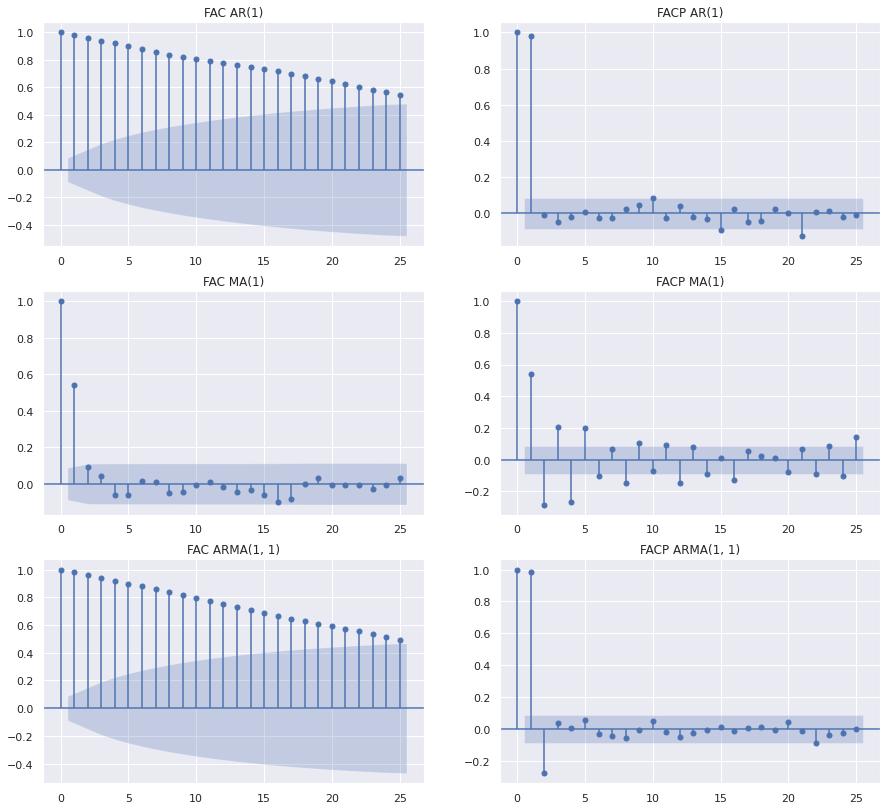
\includegraphics[width=14cm]{figuras/parciais}
\caption{Na coluna esquerda as autocorrelações e na coluna direita as autocorrelações parciais calculadas de alguns modelos $ARIMA$, demonstrando seus comportamentos esperados. Na primeira linha temos o modelo $AR(1)$, na segunda linha o modelo $MA(1)$, e na terceira linha o modelo $ARMA(1,1)$.}
\label{fig:parciais}
\end{figure}

Esta é uma clara desvantagem dos modelos paramétricos de aprendizagem, já que dependem de parâmetros que devem ser definidos \emph{a priori}, e os procedimentos para estimá-los, como neste caso, podem ser inexatos e até mesmo inconclusivos, dada a natureza complicada das funções de autocorrelação.

A recomendação dada por Morettin e Toloi \citep{morettin} é a mais comum, no âmbito de aprendizado de máquina, e consiste em testar vários parâmetros que se mostrem razoáveis após as análises feitas, e verificar qual série modelada é a mais adequada à série real de interesse, de acordo com alguma métrica de erro.